\sectionframe{The Halved Model}
\section{Halved Model}

\begin{frame}{Lifting the Model}
	\vspace{-1em}
	\begin{columns}
		\begin{column}{.4 \textwidth}
			\begin{figure}
				\includegraphics[width=\textwidth]{63_MinimalRepr_Adding_Halved/Cob_Vis_s/Manual/result.png}
			\end{figure}
		\end{column}
		\begin{column}{.5 \textwidth}
			\pause
			\begin{itemize}
				\item Lift model from $[0, 1)$ to $\mathbb{R}$ \pause
				\item The infinite model repeats every $1$ \pause
				\item But it even repeats every $\frac{1}{2}$ because of the built-in symmetry \pause
				\item Drop the model to $[0, \frac{1}{2})$ \pause
			\end{itemize}
			\begin{align*}
				x    & \mapsto g(x) \mod \frac{1}{2}                                            \\
				g(x) & = \begin{cases}
					         l(x) = a_L \cdot x^2 + b_L \cdot x + c_L & \text{ if } x < \frac{1}{4} \\
					         r(x) = b_R \cdot x + c_R                 & \text{ else}
				         \end{cases}
			\end{align*}
		\end{column}
	\end{columns}
\end{frame}

\begin{frame}{Pic}
	\todo{Picture of halved model function?}
\end{frame}

\begin{frame}{Period-adding in the Halved Model}
	\begin{figure}
		\includegraphics[width=.4 \textwidth]{63_MinimalRepr_Adding_Halved/1D_Period_1_add_hor_D1/result.png}
		\quad
		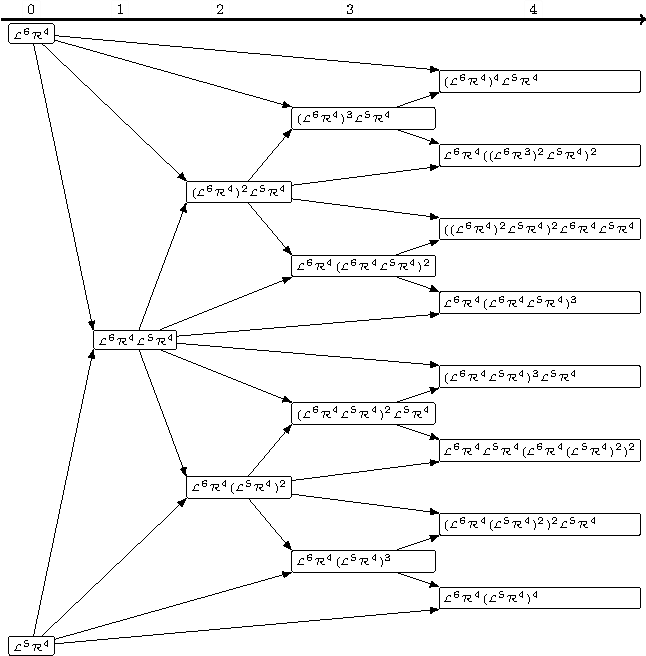
\includegraphics[width=.4 \textwidth]{../../Report/Figures/FareyTrees/Minrep_Adding1_Halved/adding.pdf}
	\end{figure}
\end{frame}

\begin{frame}{Period-adding in the Halved Model}
	\begin{itemize}
		\item Periods add up!
		\item Symbolic sequences concatenate!
	\end{itemize}
	\pause
	\vspace{3em}
	\begin{itemize}
		\item Allegory of the case (``Höhlengleichnis'') type of situation
		\item Different rules needed in full model
	\end{itemize}
\end{frame}

\begin{frame}{Some Definitions}
	\vspace{-1em}
	\begin{definition}[Syllables]
		A sequence of the same symbols is called a syllable, if there are no more of the same symbol before or after the syllable in the context of a symbolic sequence. \\
		For example $\L^3$ is a syllable of $\L^3\R^2$, but $\L^2$ is not. \\[1em]
		A pair of syllables next to each other is called a 2-syllable.
		A 4-syllable is a quadrupel of syllables next to each other.
	\end{definition}
	\begin{itemize}
		\pause
		\item A rotation in the halved model corresponds to one 2-syllable \pause
		\item A rotation in the full model corresponds to one 4-syllable \pause
		\item A rotation in the full model corresponds to 2 rotations in the halved model
	\end{itemize}
\end{frame}

\begin{frame}{Translating Symbolic Sequences 1}
	\begin{definition}[Translating 4-syllables]
		To translate a 4-syllable (2 rotations) from the halved model to one rotation in the full model, we define $t$.
		\begin{align*}
			t: \L^a\R^b\L^c\R^d \mapsto \A^a\B^b\C^c\D^d
		\end{align*}
	\end{definition}

	\pause
	From the ad-hoc method:
	\pause
	\begin{itemize}
		\item We can only translate 4-syllables (2 rotations in the halved model) at a time \pause
		\item Especially: We cannot translate a 2-syllable alone
	\end{itemize}
	\pause
	So if the cycle in the halved model has an odd number of rotations (2-syllables) we need to wrap around once while translating.
\end{frame}

\begin{frame}{The First Consequences}
	\begin{theorem}[Periods in the Full Model]
		A cycle in the halved model with period $n$ manifests as a cycle with period
		\begin{itemize}
			\item $2n$ if it has an odd number of rotations (2-syllables)
			\item $n$ if it has an even number of rotations (2-syllables)
		\end{itemize}
	\end{theorem}
	\pause
	\begin{theorem}[Coexistence in the Full Model]
		A cycle in the halved model manifests as
		\begin{itemize}
			\item a single cycle if it has an odd number of rotations
			\item 2 coexisting cycles if it has an even number of rotations
		\end{itemize}
	\end{theorem}
\end{frame}

\begin{frame}{The First Consequences}
	\todo{only rule for coexistence, write down ignore below talk about redundancy}
	From this we can formulate rules for the period and coexistence of child nodes in the farey-tree in the full model.
	\pause
	\begin{itemize}
		\item Consequences of the next theorem \pause
		\item Redundant \pause
		\item Omitted for brevity
	\end{itemize}
	\begin{theorem}{Coexistence in Child Nodes}
		\todo{necessary? if we do this we also should add rules for periods?}
	\end{theorem}
\end{frame}

\begin{frame}{Translating Symbolic Sequences}
	\todo{algo for halved -> full}
	\todo{maybe skip if not enough time}
\end{frame}

\begin{frame}{The Next Consequences}
	\begin{theorem}[Cycles in Child Nodes of two Nodes with Singular Cycles]
		The cycles $\pi^a$ and $\pi^b$ of a node with two parents with a singular cycle each, $\phi$ and $\psi$ are
		\begin{align*}
			\pi^a = \phi_1 \dots \phi_{\frac{n-1}{2}} \left[\phi_{\frac{n+1}{2}} \mid \psi_{\frac{m+1}{2}}\right] \psi_{\frac{m+3}{2}} \dots \psi_m
		\end{align*}
		and
		\begin{align*}
			\pi^b =  \phi_{\frac{n+3}{2}} \dots \phi_n \psi_1 \dots \psi_{\frac{m-1}{2}} \left[\psi_{\frac{m+1}{2}} \mid \phi_{\frac{n+1}{2}}\right]
		\end{align*}
	\end{theorem}
\end{frame}

\begin{frame}{The Next Consequences}
	\begin{theorem}[Cycles in Child Nodes of two Nodes with a Different Multiplicity of Cycles]
		The cycle $\pi$ of a node with one parent with a single cycle $\phi$ and one parent with two coexisting cycles $\psi^a$ and $\psi^b$ is either
		\begin{itemize}
			\item If $\phi$ is associated with the left parent node
			      \begin{align*}
				      \pi = \phi_1 \dots \phi_{\frac{n-1}{2}} \left[\phi_{\frac{n+1}{2}} \mid \psi_m\right] \psi_1 \dots \psi_{m-1} \left[\psi_m \mid \phi_{\frac{n+1}{2}}\right] \phi_{\frac{n+3}{2}} \dots \phi_n \psi^a
			      \end{align*}
			\item If $\phi$ is associated with the right parent node
			      \begin{align*}
				      \pi = \psi^a \phi_1 \dots \phi_{\frac{n-1}{2}} \left[\phi_{\frac{n+1}{2}} \mid \psi_m\right] \psi_1 \dots \psi_{m-1} \left[\psi_m \mid \phi_{\frac{n+1}{2}}\right] \phi_{\frac{n+3}{2}} \dots \phi_n
			      \end{align*}
		\end{itemize}
	\end{theorem}
\end{frame}

\begin{frame}
	\todo{rotation tuple rules}
	\todo{for this we need to define rotation tuples... too much?}
\end{frame}
